\documentclass[red,slidestop,notes,compress,mathserif]{beamer}

%\usepackage{beamerthemesplit}
\setbeamertemplate{navigation symbols}{}
\setbeamertemplate{note page}[plain]

\usetheme{Boadilla}
\usepackage{wasysym}
\usefonttheme{professionalfonts} % using non standard fonts for beamer
\usefonttheme{serif} % default family is serif
\usepackage{fontspec}

\usepackage{fontspec}
\newfontfamily\greekfont[Mapping=tex-text]{DejaVu Serif}
\setmainfont{Liberation Serif}


\title[ΕΜΠ, Αθήνα]{Σχεδιασμός και υλοποίηση μηχανισμών pipe και fork σε unikernels} 
\author[X. Μάινας]{Μάινας Χαράλαμπος
\vspace{.75em}
\\
Επιβλέπων: Γεώργιος Γκούμας}
\date{Μάρτιος 2019}
\logo{
\includegraphics[scale=0.05]{figures/ntua_logo.pdf}
\includegraphics[scale=0.16]{figures/cslab_logo.pdf}}

\institute[CSLab, ΕΜΠ]{%High-Performance Systems and Interconnects (HPSI),\\
Εργαστήριο Υπολογιστικών Συστημάτων \\Σχολή Ηλεκτρολόγων Μηχανικών και Μηχανικών Υπολογιστών\\Εθνικό Μετσόβιο Πολυτεχνείο\\
%Github: \url{http://github.com/{HPSI,ananos}}\\
WWW: \url{http://cslab.ece.ntua.gr/research/}\\

\includegraphics[width=1.5cm]{figures/ntua_logo.pdf}

\includegraphics[width=3.5cm]{figures/cslab_logo.pdf}\\
%\includegraphics[angle=-90,width=4.0cm]{figs/hrakleitos.pdf}\\
}


\newcommand{\ta}{\insertframenumber}

\AtBeginSubsection[]
{
  \begin{frame}
  \frametitle{Επισκόπηση}
  \tableofcontents[currentsection,currentsubsection]
  \end{frame}
}
\begin{document}


\frame{\titlepage}
\section{Εισαγωγή}
\subsection{Unikernels}

\begin{frame}
\frametitle{Εισαγωγή}
\begin{block}{Unikernels}
Εξειδικευμένες εικόνες μηχανές, με ένα μοναδικό χώρο διευθύνσεων, τα οποία κατασκευάζονται χρησιμοποιώντας library operating systems
\end{block}
\begin{block}{Αναλύοντας τον ορισμό}
\begin{itemize}
\item Εξειδικευμένες
\item Μοναδικός χώρος διευθύνσεων
\item library operating systems
\end{itemize}
\end{block}
\end{frame}

\begin{frame}
\frametitle{Typical OS vs unikernel}
\begin{figure}
\center
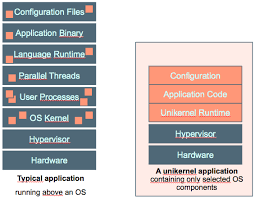
\includegraphics{figures/unikernel_vs_os.png}
\end{figure}
\end{frame}

\begin{frame}
\frametitle{Χαρακτηριστικά των unikernels}
\begin{block}{Πλεονεκτήματα}
\begin{itemize}
\item Γρήγοροι χρόνοι εκκίνησης
\item Μικρό memory footprint
\item Περισσότερη ασφάλεια
\end{itemize}
\end{block}
\begin{block}{Μειονεκτήματα}
	%%TODO: prepei na to ksanadw auto to kommati
\begin{itemize}
\item Porting
\item Μικρότερη υποστήριξη 
\end{itemize}
\end{block}
\end{frame}

\subsection{Unikernel frameworks}

\begin{frame}
\frametitle{Unikernel frameworks}
	\begin{block}{Rumprun}
		\begin{itemize}
			\item Βασισμένο στο NetBSD και συγκεκριμένα στα rump kernels 
			\item POSIX friendly
			\item Υποστήριξη για threads, filesystem
			\item Υποστηρίζει πολλές γλώσσες
			\item Πολλές εφαρμογές έτοιμες να εκτελεστούν σε αυτό
		\end{itemize}
	\end{block}
\end{frame}
\begin{frame}
\frametitle{Unikernel frameworks}
	\begin{block}{OSv}
		\begin{itemize}
			\item Φτιαγμένο από την αρχή, με στόχο την εκτέλεση στο cloud
			\item POSIX compatible
			\item Υποστήριξη για threads, filesystem
			\item Υποστηρίζει πολλές γλώσσες
			\item Πολλές εφαρμογές έτοιμες να εκτελεστούν σε αυτό
			\item Από τα πιο ενεργά projects
		\end{itemize}
	\end{block}
\end{frame}
\begin{frame}
\frametitle{Unikernel frameworks}
	\begin{block}{IncludeOS}
		\begin{itemize}
			\item Φτιαγμένο από την αρχή
			\item Μερικώς POSIX compatible
			\item Single threaded
			\item Ταχύτατα αναπτυσσόμενο project
			\item Υποστήριξη μόνο για εγαρμογές σε C++
		\end{itemize}
	\end{block}
\end{frame}
\begin{frame}
\frametitle{Unikernel frameworks}
	\begin{block}{MirageOS}
		\begin{itemize}
			\item Φτιαγμένο από την αρχή χρησιμοποιώντας OCaml
			\item Υποστήριξη μόνο για εφαρμογές σε OCaml
			\item Από τα πιο παλιά unikernel frameworks
		\end{itemize}
	\end{block}
	\pause
	\begin{block}{Πολλά ακόμα}
		\begin{itemize}
			\item ClickOS
			\item LKL
			\item Mini-OS, Unikraft
			\item HalVM, LING
		\end{itemize}
	\end{block}
\end{frame}

\subsection*{Rumprun}
\begin{frame}
\frametitle{Rumprun}
\begin{block}{Anykernels}
	Codebase (πυρήνα) όπου οι οδηγοί μπορούν να εξαχθούν και να ενσωματωθούν σε οποιοδήποτε μοντέλο ΛΣ
\end{block}
\begin{block}{Rump kernels}
	παρέχουν drivers του NetBSD ως φορητά εξαρτήματα με τα οποία μπορούμε να εκτελέσουμε εφαρμογές χωρίς να ναι απαραίτητη η ύπαρξη ΛΣ
\end{block}
\begin{figure}
\center
	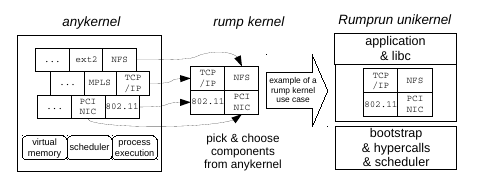
\includegraphics[scale=0.5]{figures/from_anykernel_to_rump.png}
\end{figure}
\end{frame}

\begin{frame}
\frametitle{Rumprun stack}
\begin{figure}
\center
	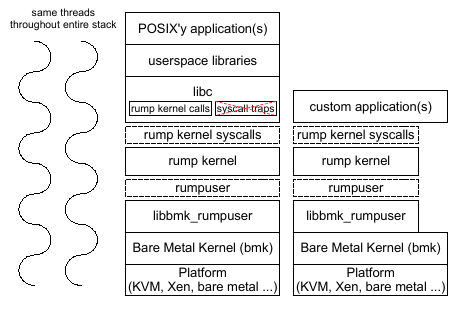
\includegraphics[scale=0.5]{figures/rumprun_stack.png}
\end{figure}
\end{frame}

\subsection{Βασική ιδέα}
\begin{frame}
\frametitle{Βασική ιδέα}
\begin{block}{single process}
\begin{itemize}
\item Βασικό κοινό χαρακτηριστικό όλων των unikernels: single process
\item Δεν υποστηρίζεται η κλήση fork
\end{itemize}
\end{block}
\begin{block}{Ιδέα}
\begin{itemize}
\item POSIX friendly 
\item Διατήρηση βασικών χαρακτηριστικών unikernels
\item Unikernels ως διεργασίες και hypervisor ως λειτουργικό συτημα
\end{itemize}
\end{block}
\end{frame}

\begin{frame}
\frametitle{Αντικείμενο διπλωματικής}
\begin{block}{Μηχανισμός fork}
\begin{itemize}
\item Αντί για δημιουργία νέας διεργασίας στο υπάρχον unikernel
\item Δημιουργία νέου unikernel
\item Από το επίπεδο των διεργασιών στο επίπεδο των εικονικών μηχανών
\end{itemize}
\end{block}
\begin{block}{Μηχανισμός pipe}
\begin{itemize}
\item Επικοινωνία μεταξύ δύο διεργασιών
\item Συνήθης πρακτική, pipe
\item Κατασκευή ενός μηχανισμού pipe σε επίπεδο εικονικών μηχανών. 
\end{itemize}
\end{block}
\end{frame}

\section{Μηχανισμός pipe}
\subsection{Γενική εικόνα}

\begin{frame}
\frametitle{Γενική εικόνα}
\begin{block}{Pipe system call}
int pipe(int fildes[2]); \\
Pipe semantics:
\begin{itemize}
\item Αν το pipe είναι άδειο, η κλήση ανάγνωσης μπλοκάρει μέχρι να προκύψουν δεδομένα
\item Αν το pipe είναι γεμάτο, η κλήση εγγραφής μπλοκάρει μέχρι να ελευθερωθεί χώρος
\item Αν δεν υπάρχουν ανοιχτά άκρα εγγραφής, τότε η ανάγνωση στο pipe επιστρέφει 0, end of file
\item Αν δεν υπάρχουν ανοιχτά άκρα ανάγνωσης, τότε εγγραφή στο pipe επιστρέφει το error EPIPE
\end{itemize}
\end{block}
\end{frame}

\begin{frame}
\frametitle{Γενική εικόνα}
\begin{block}{Pipe σε unikernels}
Χρήση του pipe για unikernels, όπως και στις διεργασίες ενός συμβατικού ΛΣ.
\end{block}
\begin{block}{Τρία στάδια υλοποίησης}
\begin{enumerate}
\item function call (sockets)
\item system call (sockets)
\item system call (κοινή μνήμη)
\end{enumerate}
\end{block}
\end{frame}

\subsection{Πρώτο στάδιο υλοποίησης}

\begin{frame}
\frametitle{Πρώτο στάδιο υλοποίησης}
\begin{block}{function call}
\begin{itemize}
\item Στον κώδικα της εφαρμογής
\item Δημιουργία δύο sockets (TCP)
\item Επιστροφή των δύο sockets
\item Διεύθυνση παραλήπτη
\item Δεν υλοποιήθηκαν όλα τα semantics του pipe 
\end{itemize}
\end{block}
\end{frame}

\subsection{Δεύτερο στάδιο υλοποίησης}

\begin{frame}
\frametitle{Δεύτερο στάδιο υλοποίησης}
\begin{block}{system call}
\begin{itemize}
\item Χρήση UDP sockets, αντί για TCP
\item Δημιουργία system call για τον πυρήνα του NetBSD
\item Δημιουργία δύο sockets
\item Επιστρέφονται δύο file descriptors
\item ioctl κλήση, για τη διεύθυνση του παραλήπτη
\item Δεν υλοποιήθηκαν όλα τα semantics του pipe 
\end{itemize}
\end{block}
\end{frame}

\subsection{Τρίτο στάδιο υλοποίησης}
\begin{frame}
\frametitle{Τρίτο στάδιο υλοποίησης}
\begin{block}{system call}
\begin{itemize}
\item Χρήση κοινής μνήμης μεταξύ των εικονικών μηχανών (ivshmem - nahanni)
\item Επιστρέφονται δύο file descriptors
\item Ίδιος host
\item Υλοποιήθηκαν όλα τα semantics του pipe 
\end{itemize}
\end{block}
\end{frame}

\begin{frame}
\frametitle{Τρίτο στάδιο υλοποίησης}
\begin{block}{ivshmem}
\begin{itemize}
\item Χρήση του μηχανισμού ivshmem - nahanni
\item Κοινή μνήμη μεταξύ δύο εικoνικών μηχανών σε QEMU
\item PCI driver 
\end{itemize}
\end{block}
\begin{block}{Υλοποίηση}
\begin{itemize}
\item PCI driver 
\item Pipe system call 
\end{itemize}
\end{block}
\end{frame}

\begin{frame}
\frametitle{Τρίτο στάδιο υλοποίησης}
\begin{block}{Υλοποίηση}
\begin{itemize}
\item PCI driver 
\item Pipe system call 
\end{itemize}
\end{block}
\begin{figure}
\center
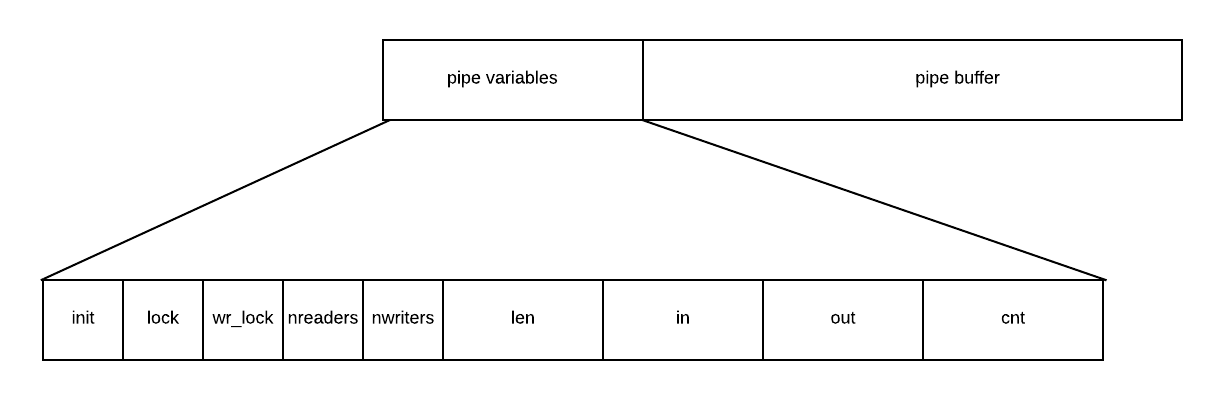
\includegraphics[scale=0.66]{figures/shared_memoery_layout.png}
\end{figure}
\end{frame}

\begin{frame}
\frametitle{Τρίτο στάδιο υλοποίησης}
\begin{columns}
\column{.4\textwidth}
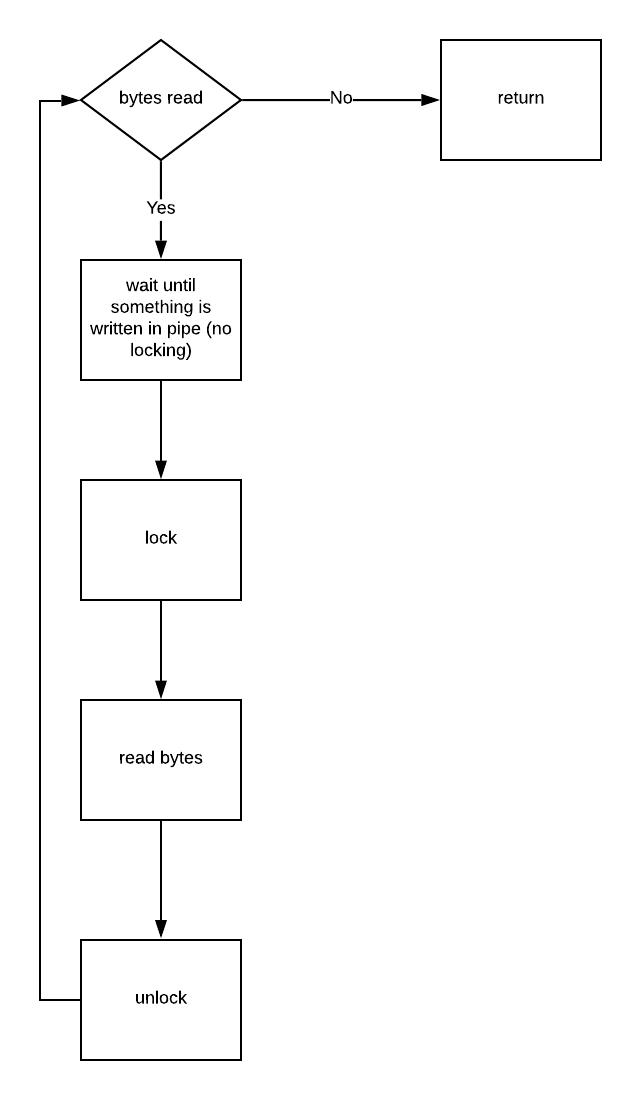
\includegraphics[scale=0.4]{figures/pipe_read.png}
\column{.4\textwidth}
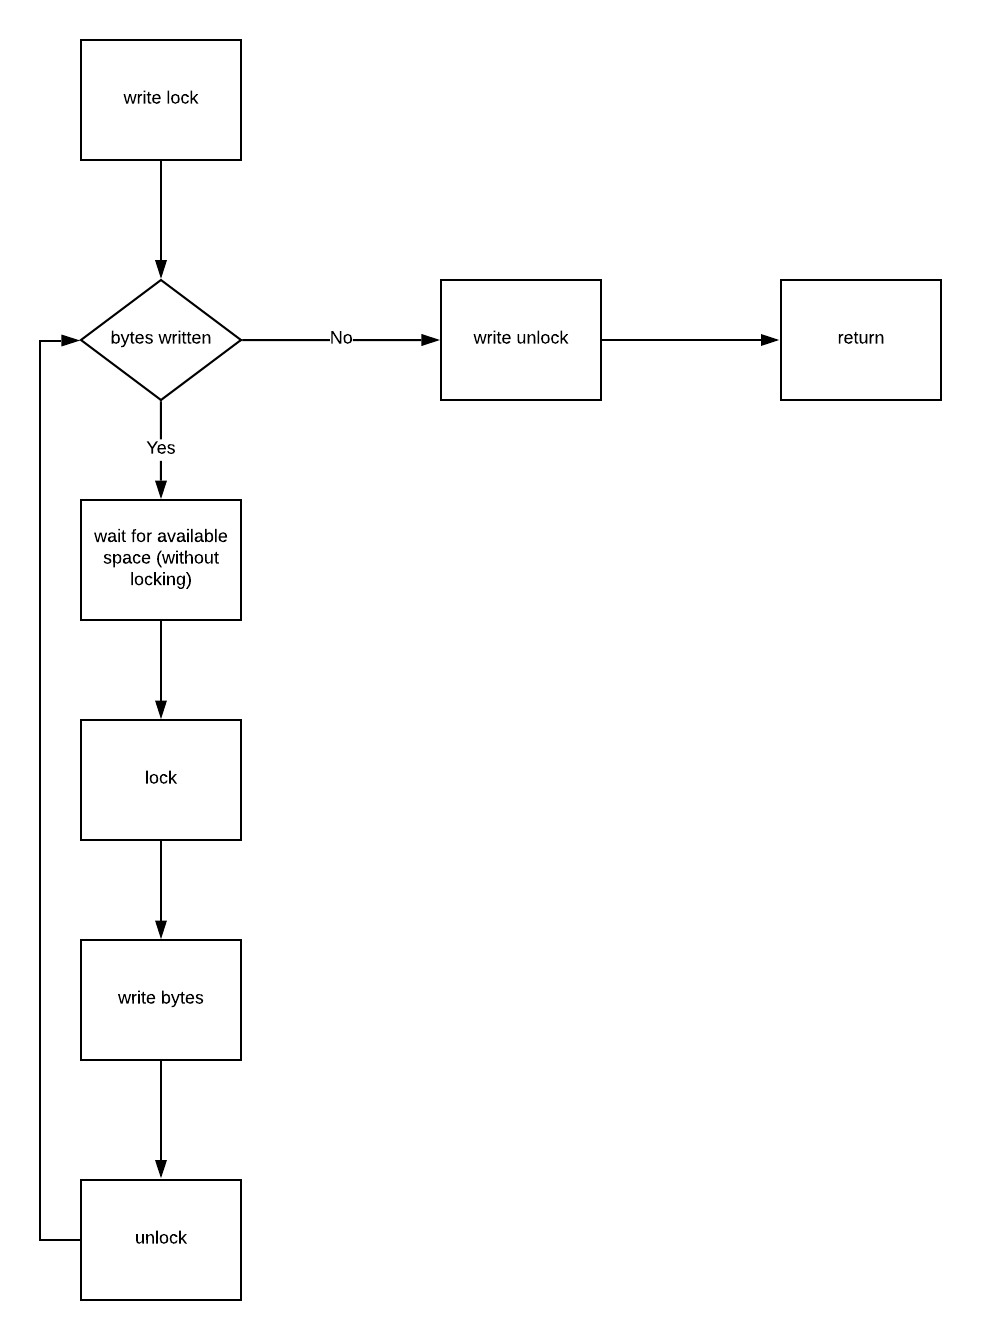
\includegraphics[scale=0.4]{figures/pipe_write.png}
\end{columns}
\end{frame}

\section{Μηχανισμός fork}
\subsection{Γενική εικόνα}
\begin{frame}
\frametitle{Γενική εικόνα}
\begin{block}{fork system call}
\begin{itemize}
\item Δημιουργία νέας διεργασίας
\item Η νέα διεργασία είναι ίδια με τη διεργασία γονέα
\item Διαχωρισμός των δύο διεργασιών με τιμή επιστροφής από την κλήση συστήματος
\item Διατήρηση ανοιχτών file descriptors στη διεργασία παιδί.
\end{itemize}
\end{block}
\end{frame}

\begin{frame}
\frametitle{fork σε συμαβατικά ΛΣ}
\begin{figure}
\center
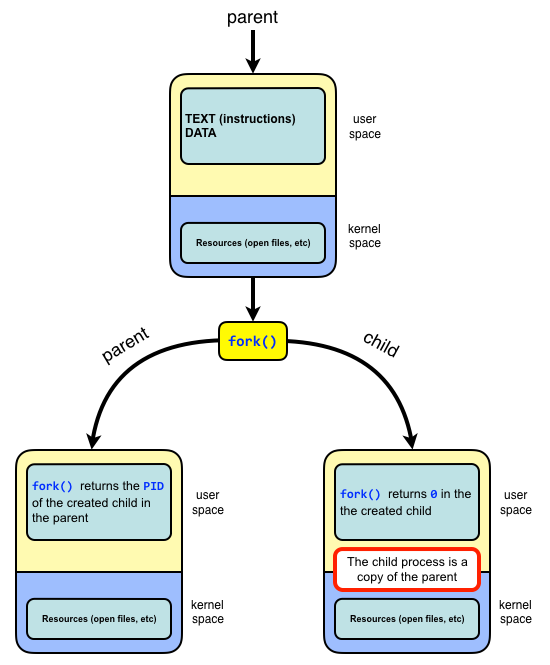
\includegraphics[scale=0.3]{figures/fork-details.png}
\end{figure}
\end{frame}

\begin{frame}
\frametitle{Γενική εικόνα}
\begin{block}{fork system call}
\begin{itemize}
\item Δημιουργία νέας διεργασίας
\item Η νέα διεργασία είναι ίδια με τη διεργασία γονέα
\item Διαχωρισμός των δύο διεργασιών με τιμή επιστροφής από την κλήση συστήματος
\item Διατήρηση ανοιχτών file descriptors στη διεργασία παιδί.
\end{itemize}
\end{block}
\begin{block}{Στόχος}
Μεταφορά της ίδιας λειτουργίας σε επίπεδο εικονικών μηχανών
\end{block}
\end{frame}

\begin{frame}
\frametitle{unikernel fork}
\begin{figure}
\center
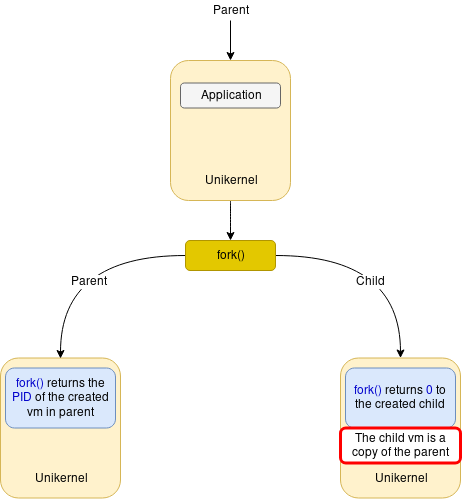
\includegraphics[scale=0.4]{figures/unikernel_fork.png}
\end{figure}
\end{frame}

\begin{frame}
\frametitle{Γενική εικόνα}
\begin{block}{Υλοποίηση}
\begin{itemize}
\item Μηχανισμός migration του QEMU
\item hypercalls 
\end{itemize}
\end{block}
\begin{block}{Βήματα}
\begin{itemize}
\item Ενημέρωση των κοινών μεταβλητών του pipe (αν υπάρχει pipe)
\item Εκκίνηση διαδικασίας migration
\item Αναμονή για migration
\item Εκκίνηση νέας εικονικής μηχανής με βάση το migration file
\item Συγχρονισμός κοινής μνήμης
\end{itemize}
\end{block}
\end{frame}

\subsection{Βήματα}

\begin{frame}
\frametitle{Ενημέρωση κοινών μεταβλητών στο pipe}
\begin{itemize}
\item Αν υπάρχει pipe θα πρέπει να ενημερωθούν οι κοινές μεταβλητές
\item Έλεγχος ύπαρξης pipe
\item Αύξηση των μετρητών ανοιχτών άκρων
\item Πρόσβαση στην κοινή μνήμη
\end{itemize}
\end{frame}

\begin{frame}
\frametitle{Εκκίνηση δημιουργίας migration file}
\begin{block}{Από τη μεριά του rumprun}
Hypercall για την εκκίνηση δημιουργίας migration file
\end{block}
\begin{block}{Από τη μεριά του QEMU}
\begin{itemize}
\item Χρήση του μηχανισμού migration
\item Migration thread
\item Λειτουργία της εικονικής μηχανής γονέας
\end{itemize}
\end{block}
\end{frame}

\begin{frame}
\frametitle{Εκκίνηση δημιουργίας migration file}
\begin{figure}
\center
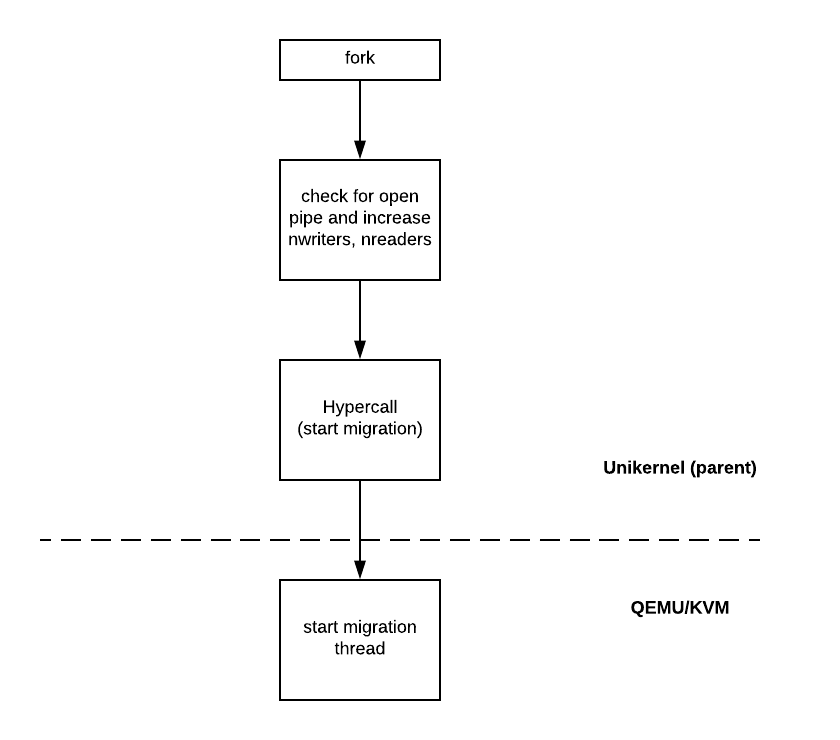
\includegraphics[scale=0.57]{figures/fork_stage1.png}
\end{figure}
\end{frame}

\begin{frame}
\frametitle{Αναμονή για την περάτωση του migration}
\begin{block}{Από τη μεριά του rumprun}
\begin{itemize}
\item Busy wait 
\item Σημείο εκκίνησης του unikernel παιδί.
\end{itemize}
\end{block}
\begin{block}{Από τη μεριά του QEMU}
\begin{itemize}
\item Κατάσταση του migration thread
\item Hypercalls counter
\end{itemize}
\end{block}
\end{frame}

\begin{frame}
\frametitle{Αναμονή για την περάτωση του migration}
\begin{block}{Hypercalls counter}
\begin{itemize}
\item Διάκριση παιδιού, γονέα
\item Διαφορετικοί counters για κάθε vm
\item Migration, χρονοβόρα διαδικασία
\item Ένα ακριβώς hypercall από το παιδί
\end{itemize}
\end{block}
\end{frame}

\begin{frame}
\frametitle{Αναμονή για την περάτωση του migration}
\begin{figure}
\center
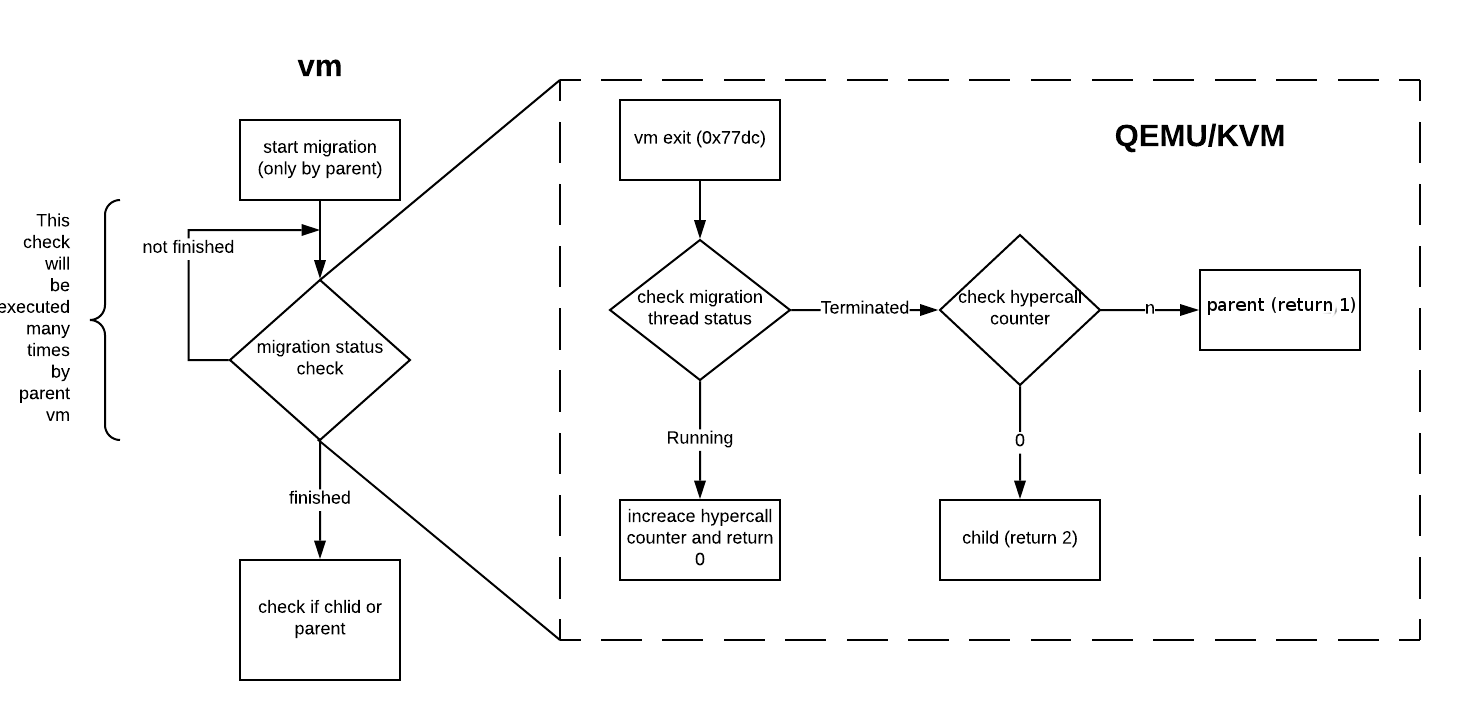
\includegraphics[scale=0.57]{figures/check_migration_status.png}
\end{figure}
\end{frame}

\begin{frame}
\frametitle{Δημιουργία νέας εικονικής μηχανής}
\begin{block}{Από τη μεριά του rumprun}
Hypercall για την εκκίνηση νέας εικονικής μηχανής
\end{block}
\begin{block}{Από τη μεριά του QEMU}
\begin{itemize}
\item fork 
\item Επιστροφή process id 
\item Εκκίνηση νέας εικονικής μηχανής 
\end{itemize}
\end{block}
\end{frame}

\begin{frame}
\frametitle{Εκκίνηση δημιουργίας migration file}
\begin{figure}
\center
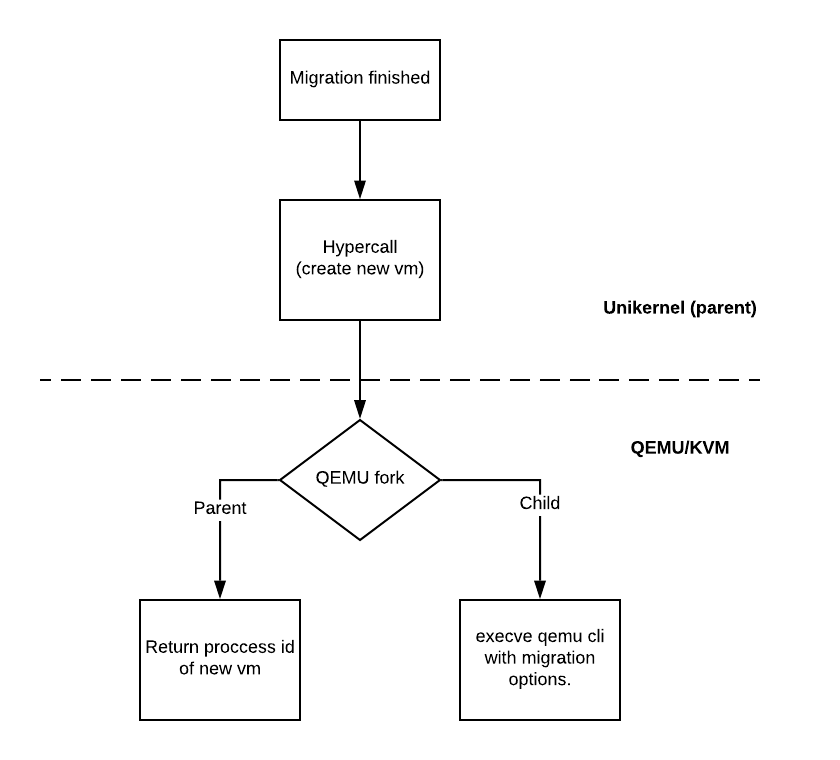
\includegraphics[scale=0.57]{figures/fork_stage2.png}
\end{figure}
\end{frame}

\begin{frame}
\frametitle{Συγχρονισμός εικονικής μνήμης}
\begin{itemize}
\item Μόνο στην περίπτωση χρήσης pipe
\item Bug(?) κοινής μνήμης
\item Busy wait από το γονιό
\item Εγγραφή στην κοινή μνήμη από το παιδί
\end{itemize}
\end{frame}

\begin{frame}
\frametitle{Όλα τα βήματα}
\begin{figure}
\center
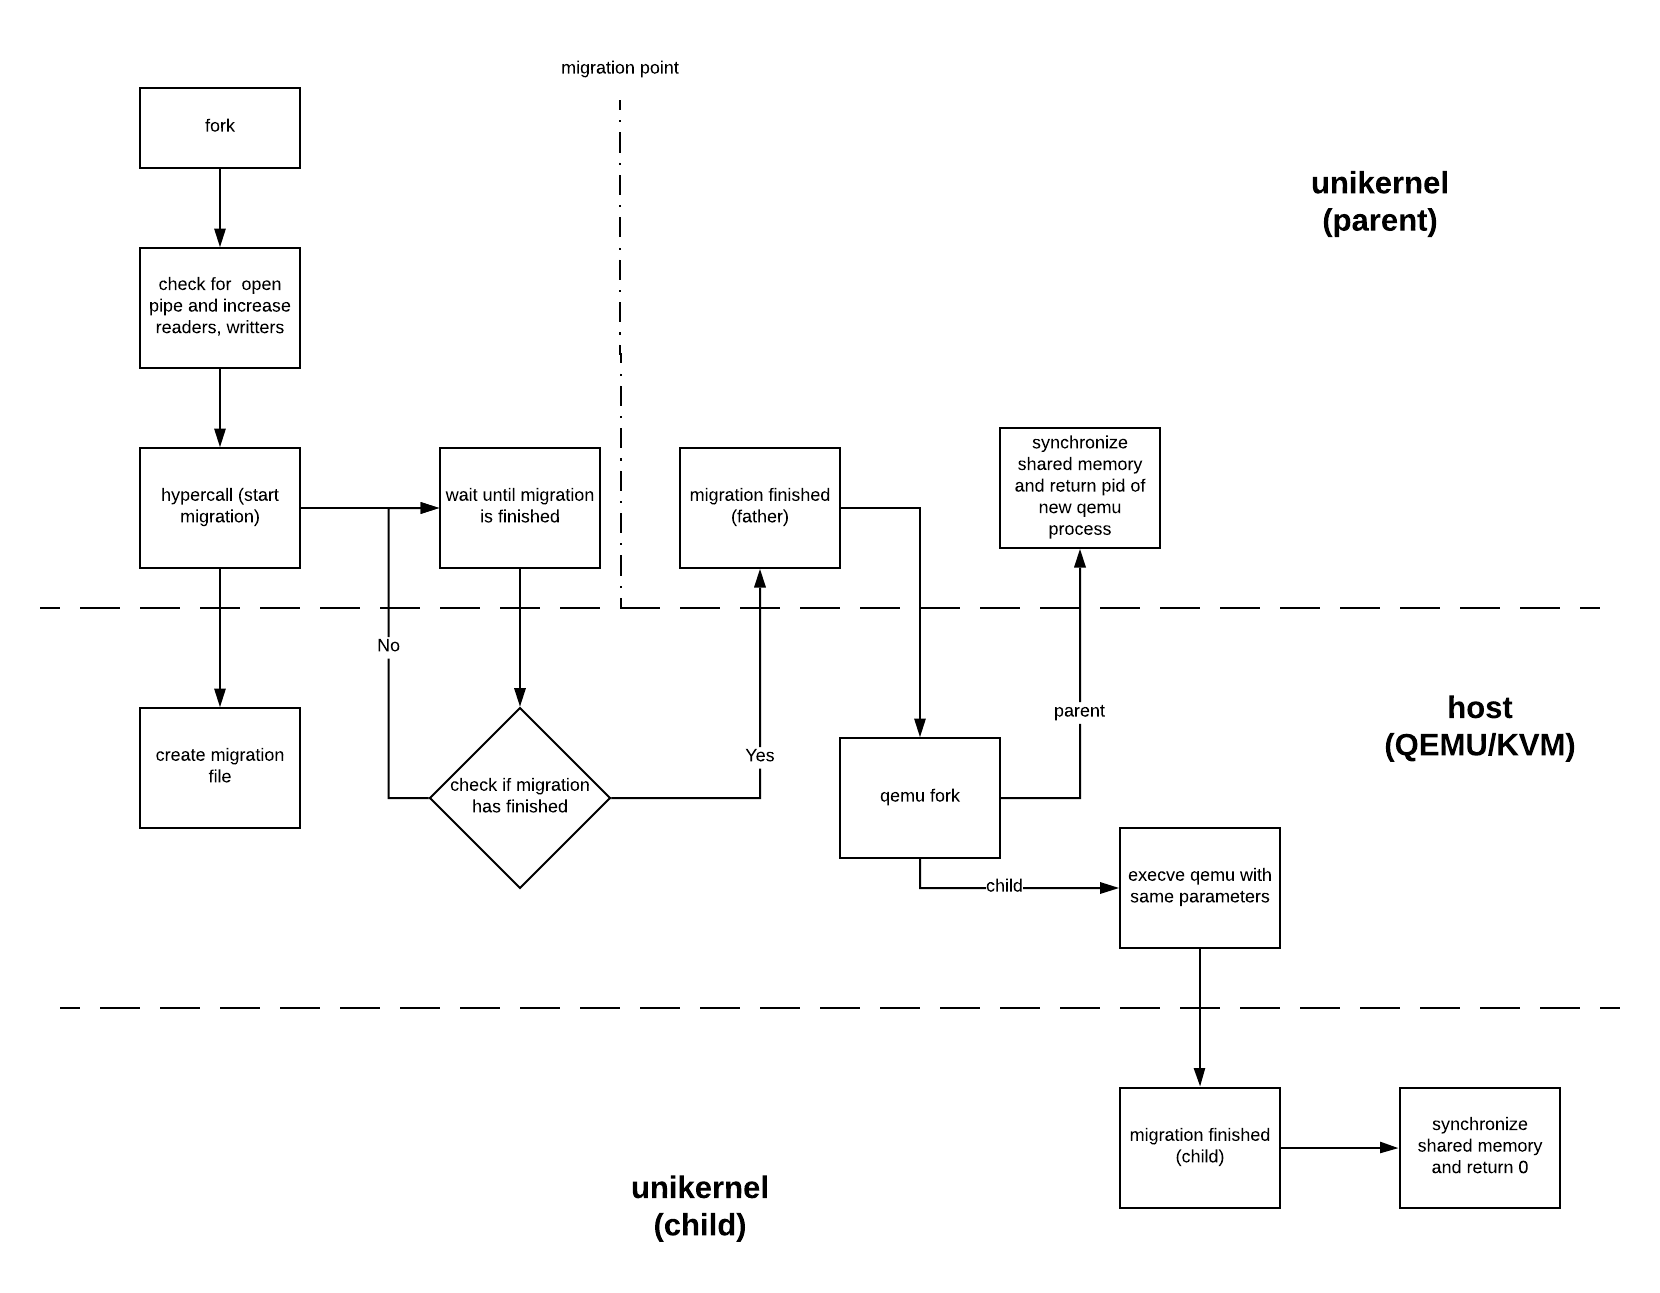
\includegraphics[scale=0.38]{figures/fork_olo.png}
\end{figure}
\end{frame}

\begin{frame}
\frametitle{Όλα τα βήματα}
\begin{figure}
\center
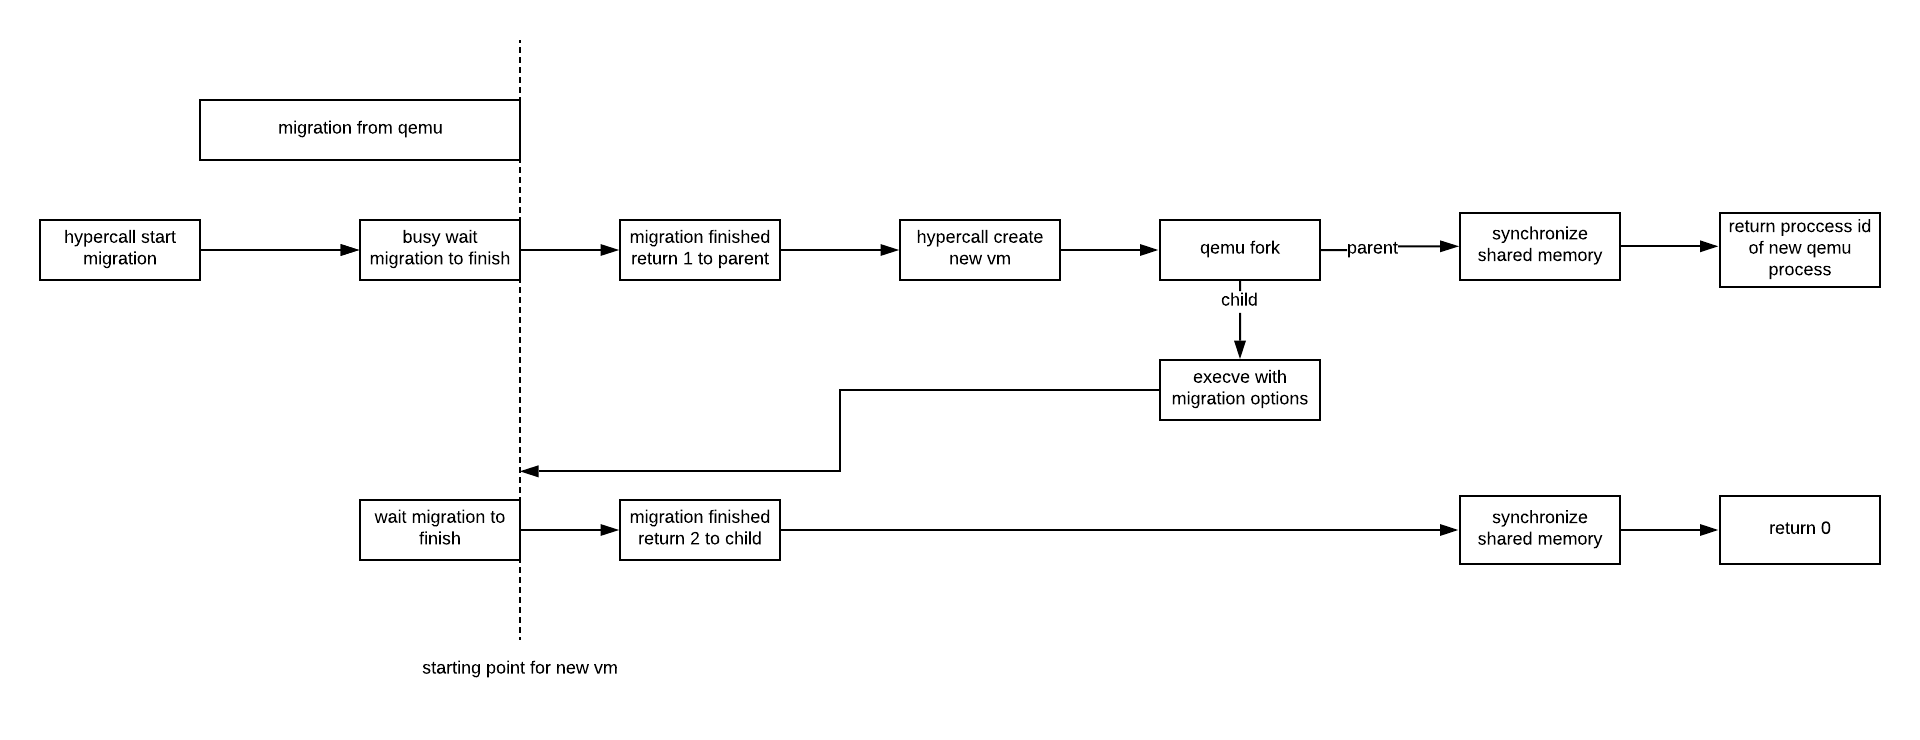
\includegraphics[scale=0.4]{figures/fork_timeline.png}
\end{figure}
\end{frame}

\subsection{Αξιολόγηση}
\begin{frame}
\frametitle{Μετρήσεις}
\begin{block}{Σύγκριση fork}
\begin{itemize}
\item Σύγκριση fork σε linux πυρήνα και του δικού μας fork 
\item Σε ίδια έκδοση QEMU (2.11.2)
\item Linux 4.9.0-7-amd64 \#1 SMP Debian 4.9.110-3+deb9u2
\item Linux: 0.541ms, Unikernel: 137,423ms
\item Διαφορά
\end{itemize}
\end{block}
\end{frame}

\begin{frame}
\frametitle{Time for each step in fork}
\begin{figure}
\center
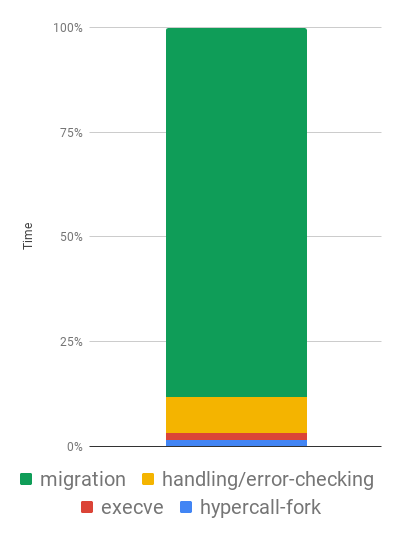
\includegraphics[scale=0.6]{figures/fork_breakdown.png}
\end{figure}
\end{frame}

\section*{Επίλογος}

\subsection*{Σύνοψη}

\begin{frame}
\frametitle{Σύνοψη}
Unikernels:
\begin{itemize}
\item Ενδιαφέρουσα τεχνολογία
\item Διαφορετικοί στόχοι 
\item POSIX compatible
\item Single process
\end{itemize}
\begin{block}{Αντιμετόπιση των unikernels ως διεργασίες}
\begin{itemize}
\item Μηχανισμός pipe για unikernels σε ίδιο και διαφορετικό host
\item Μηχανισμός fork για unikernels σε ίδιο host
\end{itemize}
\end{block}
%\end{block}
\end{frame}

\begin{frame}
\frametitle{Μελλοντικές Επεκτάσεις}
\begin{itemize}
\item Χρήση σημάτων, για τη βελτίωση του μηχνασιμού pipe
\item Επέκταση inter-unikernel μηχανισμών επικοινωνίας 
\item Βελτίωση μηχανισμού fork
\item Επέκταση του μηχανισμού και σε άλλες πλατφόρμες.
\end{itemize}
%%Διαθέσιμο στο \url{https://github.com/HPSI/v4v}

\end{frame}
%
\begin{frame}
\frametitle{Ευχαριστώ!}
                \vfill%
\begin{columns}
        \column{.35\textwidth}
        \begin{center}
                %\vfill%
            %    \begin{block}{}
        \begin{center}
                        {\LARGE Ερωτήσεις;}
        \end{center}
             %   \end{block}
                \vfill%
                %\vfill%
        \end{center}
\end{columns}
                \vfill%
\end{frame}


\begin{frame}
\frametitle{}
                \vfill%
\begin{columns}
        \column{.35\textwidth}
        \begin{center}
                %\vfill%
            %    \begin{block}{}
             %   \end{block}
                \vfill%
                %\vfill%
        \end{center}
\end{columns}
                \vfill%
\end{frame}
%
\begin{frame}
\frametitle{}
                \vfill%
\begin{columns}
        \column{.35\textwidth}
        \begin{center}
                %\vfill%
            %    \begin{block}{}
        \begin{center}
                        {\LARGE Backup}
        \end{center}
             %   \end{block}
                \vfill%
                %\vfill%
        \end{center}
\end{columns}
                \vfill%
\end{frame}

%%\begin{frame}
%%\frametitle{Πειραματική αποτίμηση -- 2M message size vs Hypercalls}
%%\begin{columns}
%%\column{.8\textwidth}
%%\includegraphics[width=\textwidth]{figures/2M.eps}
%%\end{columns}
%%\end{frame}
%%
%%\begin{frame}
%%\frametitle{Πειραματική αποτίμηση -- Datagram scale}
%%\begin{columns}
%%\column{.8\textwidth}
%%\includegraphics[width=\textwidth]{figures/bw_dgram_scale.eps}
%%\end{columns}
%%\end{frame}
%%
%%\begin{frame}
%%\frametitle{Πειραματική αποτίμηση -- Hypercalls per message}
%%\begin{columns}
%%\column{.8\textwidth}
%%\includegraphics[width=\textwidth]{figures/mix.eps}
%%\end{columns}
%%\end{frame}
%
%\begin{frame}
%\frametitle{Πειραματική αποτίμηση -- Ποσοστό χρήσης CPU για το VM}
%\begin{columns}
%\column{.8\textwidth}
%\includegraphics[width=\textwidth]{figs/bare/lat_breakdown_domU.eps}
%\end{columns}
%\end{frame}
%
%\begin{frame}
%\frametitle{Xen2MX -- I}
%\begin{columns}
%\column{.8\textwidth}
%\includegraphics[width=\textwidth]{figs/bare/xen2mx_step1.pdf}
%\end{columns}
%\end{frame}
%
%\begin{frame}
%\frametitle{Xen2MX -- II}
%\begin{columns}
%\column{.8\textwidth}
%\includegraphics[width=\textwidth]{figs/bare/xen2mx_step2.pdf}
%\end{columns}
%\end{frame}
%
%\begin{frame}
%\frametitle{Xen2MX -- III}
%\begin{columns}
%\column{.8\textwidth}
%\includegraphics[width=\textwidth]{figs/bare/xen2mx_step3.pdf}
%\end{columns}
%\end{frame}
%
%\begin{frame}
%\frametitle{Xen2MX -- IV (Bridged)}
%\begin{columns}
%\column{.8\textwidth}
%\includegraphics[width=\textwidth]{figs/bare/xen2mx_step4.pdf}
%\end{columns}
%\end{frame}
%
%\begin{frame}
%\frametitle{Xen2MX -- ΙV (IOV)}
%\begin{columns}
%\column{.8\textwidth}
%\includegraphics[width=\textwidth]{figs/bare/xen2mx_step5.pdf}
%\end{columns}
%\end{frame}
%
%\begin{frame}
%\frametitle{Xen2MX -- IV (Xen2MX)}
%\begin{columns}
%\column{.8\textwidth}
%\includegraphics[width=\textwidth]{figs/bare/xen2mx_step6.pdf}
%\end{columns}
%\end{frame}
%

\end{document}
